% Compile with pdfLaTeX, BibTeX, and pdfLaTeX twice.
\documentclass[11pt,a4paper]{article}
\usepackage[T1]{fontenc}
\usepackage[margin=2.3cm]{geometry}
\usepackage{amsmath,amssymb,bm,graphicx,booktabs,float}
\usepackage{algorithm,algpseudocode,listings,xcolor}
\usepackage[hidelinks]{hyperref}
\setlength{\emergencystretch}{2em}
\lstset{language=Python,basicstyle=\ttfamily\footnotesize,breaklines=true,
frame=single,showstringspaces=false,keywordstyle=\color{blue!60!black},
commentstyle=\color{green!40!black},numbers=left,numberstyle=\tiny}
\title{Project 2, Direction 3\\Algorithm and Implementation}
\author{Material for integration with the supplied Method section}
\date{5 November 2026}
\begin{document}
\maketitle
\setcounter{section}{2}
\section{Algorithm and Implementation}
\label{sec:algorithm_impl}

The implementation translates the conservative stencil and conforming weak form in the Method section into sparse linear systems. It follows the verification and matched-comparison requirements of the course brief and problem pack \cite{projectbrief,problempack}. FDM is the core discretisation. A two-dimensional triangular $\mathcal P_1$ FEM implementation supplies the depth comparison already specified in the Method section. Both use NumPy arrays and SciPy sparse algebra \cite{harris2020numpy,virtanen2020scipy}.

\begin{figure}[H]
\centering
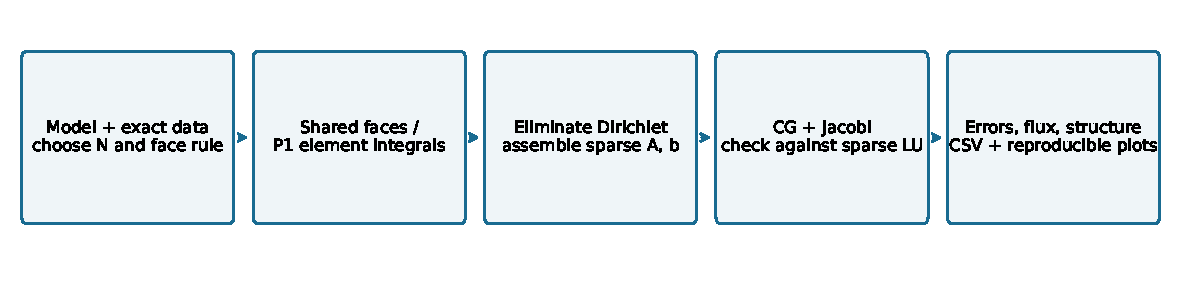
\includegraphics[width=\linewidth]{figures/fig01_algorithm.pdf}
\caption{Computational path from the continuous data to independently checked numerical output. The direct solve and the iterative solve act on the same assembled matrix and right-hand side.}
\label{fig:alg_flow}
\end{figure}

\subsection{Data layout and conservative FDM assembly}
The unit square is divided into $N$ intervals per coordinate, with $h=1/N$ and $n=N-1$ interior points. The code uses \texttt{indexing='ij'} and C-order flattening, so
\[
k=(i-1)n+(j-1),\qquad 1\leq i,j\leq n.
\]
The $y$ coordinate varies fastest. East/west connections have offsets $\pm n$ and north/south connections have offsets $\pm1$. Separate two-dimensional masks define these connections, preventing a spurious wrap between adjacent grid columns.

Each physical edge coefficient is computed once. The smooth benchmark uses arithmetic averages of neighbouring nodal coefficients. The layered benchmark uses odd $N$ so the interface bisects an edge, and compares arithmetic against harmonic averages. After division by $h^2$, the same edge weight is inserted into the two transposed off-diagonal positions. The diagonal retains all four outgoing weights. A boundary neighbour contributes $+a_fg/h^2$ to the right-hand side. Only interior unknowns enter the matrix.

\begin{algorithm}[H]
\caption{Vectorised conservative FDM assembly}
\begin{algorithmic}[1]
\Require $N$, coefficient and source functions, Dirichlet data, face rule
\Ensure Interior CSR matrix $A$ and right-hand side $b$
\State Sample $a$, $f$ and $g$ on the prescribed grid
\State Form shared $x$-edge and $y$-edge coefficients
\State Form the $(N-1)\times(N-1)$ interior index array
\State Add the diagonal sum of four face weights
\State Add each interior connection in both matrix directions
\State Add known boundary contributions to $b$
\State Construct COO arrays and convert to CSR
\State Check symmetry, diagonal signs and off-diagonal signs
\end{algorithmic}
\end{algorithm}

The exact FDM nonzero count is $5n^2-4n$, and assembly and matrix-vector products require $\mathcal O(n^2)$ storage and work. The unit test at $N=3$ checks the hand-derived $4\times4$ constant-coefficient matrix. A second test checks the coefficient $-N^2(20/11)$ in a row adjacent to the material interface. Together they check the ordering, scaling and special interface row.

\lstinputlisting[firstline=63,lastline=74,caption={The actual vectorised COO assembly in \texttt{src/discretisation.py}. Each interior connection contributes a symmetric pair.}]{src/discretisation.py}

\begin{figure}[H]
\centering
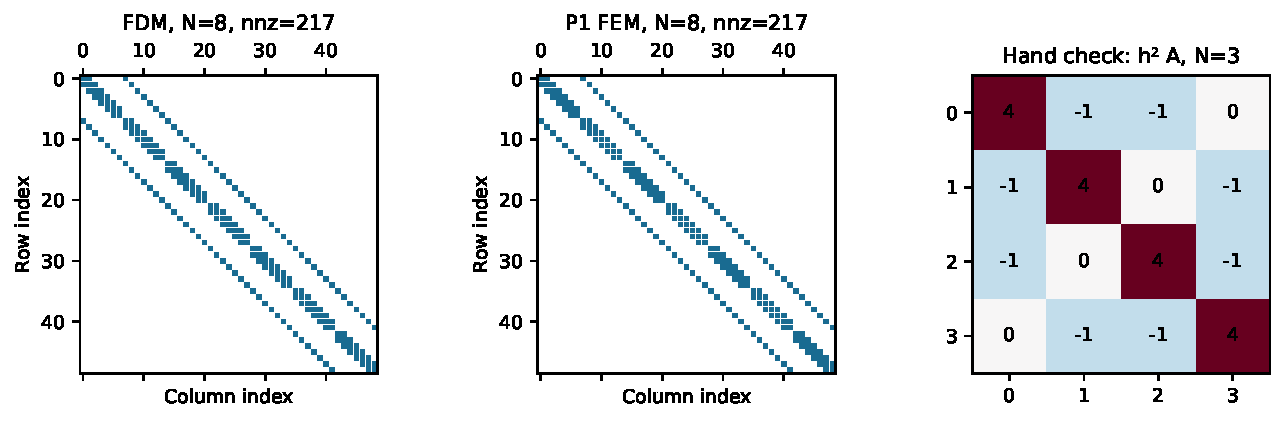
\includegraphics[width=0.96\linewidth]{figures/fig02_sparse_assembly.pdf}
\caption{Actual matrix patterns and the hand-check matrix. With this right-triangle mesh, zero cross-diagonal element couplings are removed from sparse storage. Similar sparsity patterns alone do not establish equality of the FDM and FEM operators or loads.}
\label{fig:alg_spy}
\end{figure}

\subsection{Linear solvers, residuals and measured cost}
Symmetric Dirichlet elimination and positive conductances give the SPD structure required by conjugate gradients. The main comparison uses CG with zero initial guess and Jacobi inverse preconditioner $M=\operatorname{diag}(A)^{-1}$, with the same requested tolerance for both discretisations. SciPy's interface checks
\[
\|b-AU\|_2\leq\max(\mathrm{rtol}\|b\|_2,\mathrm{atol}),
\qquad \mathrm{rtol}=10^{-12},\quad\mathrm{atol}=0.
\]
The code explicitly recomputes the residual after CG exits. If round-off in the recursively updated residual leaves the recomputed residual above the target, it solves a residual-correction system and adds the correction. At most three corrections are allowed. The final explicit check permits a 10\% floating-point margin on the requested tolerance; failure raises an error. Correction iterations and work enter the reported CG totals.

A sparse SuperLU factorisation supplies an independent solution of the same system. The code calls \texttt{splu} on a CSC matrix with COLAMD ordering, then applies the factorisation to $b$. This separates factorisation from triangular-solve cost. It also reports
\[
\eta_\infty=
\frac{\|b-AU\|_\infty}{\|A\|_\infty\|U\|_\infty+\|b\|_\infty},
\qquad
\delta_{\rm alg}=\|U_{\rm CG}-U_{\rm LU}\|_\infty.
\]
The independent solution difference measures the solver contribution relative to the observed discretisation error. A small residual is supported by this solution check.

Assembly, preconditioner setup, CG, LU factorisation and triangular solves are timed separately with \texttt{perf\_counter}. Timings use three serial repetitions, and each reported stage is its median. Numerical thread pools are limited to one thread. Diagnostic residual histories, quadrature error evaluation, eigenvalue estimation, file writing and plotting lie outside the reported main-solve timings. The cost--accuracy plot uses assembly plus Jacobi setup plus CG. Environment versions, source hashes and all individual timing repetitions accompany the tables.

\subsection{Two-dimensional P1 FEM and matched settings}
Each Cartesian square is split along the lower-left to upper-right diagonal. Three vertex indices describe each triangle. The constant local basis gradients are obtained from the affine triangle map, and the code assembles
\[
K_{ij}^{T}=(\nabla\varphi_i\cdot\nabla\varphi_j)\int_T a\,dx,
\qquad b_i^T=\int_Tf\varphi_i\,dx.
\]
This implementation uses explicit NumPy element arrays and SciPy assembly. A $5\times5$ Gauss--Legendre rule under a Duffy map evaluates the triangle integrals. With reference coordinates $r,s\in(0,1)$, the barycentric coordinates are $((1-r)(1-s),r,(1-r)s)$ and the Jacobian factor is $1-r$. The reference weights sum to $1/2$. For the affine smooth coefficient and for an aligned piecewise-constant coefficient, this rule integrates stiffness coefficients exactly up to round-off. A higher quadrature order independently checks the smooth load and error integral on a representative mesh.

Local $3\times3$ matrices are accumulated in COO format, converted to CSR and duplicate entries summed. With boundary vertex set $B$ and interior set $I$, Dirichlet data are imposed through
\[
K_{II}U_I=b_I-K_{IB}g_B.
\]
The raw FEM flux is $-a\nabla u_h$ on each triangle. Its one-sided normal traces are evaluated from the actual neighbouring elements. Conforming P1 functions are continuous, while their raw normal fluxes generally jump. The particular aligned layered solution belongs to the finite-element space, permitting a separate exactness check.

The smooth comparison uses $N=16,32,64,128$, identical data, common vertices, identical CG stopping settings, and the same Jacobi construction. Each method has $(N-1)^2$ unknowns. The named nodal errors are
\[
E_{2,h}=h\left(\sum_{i,j\in I}|U_{ij}-u_*(x_i,y_j)|^2\right)^{1/2},
\qquad E_\infty=\max_{i,j}|U_{ij}-u_*(x_i,y_j)|.
\]
The code additionally evaluates a common continuous $L^2$ error. Both nodal solutions are reconstructed using P1 interpolation on the same triangles and integrated against the exact solution with a $6\times6$ Duffy quadrature rule. This explicitly defines how a nodal FDM solution enters a continuous-norm comparison. Successive-grid rates use the actual ratio of mesh widths; fitted rates use the last three meshes.

For the layered structural check, FDM uses $N=31,63,127,255$, while interface-fitted FEM uses $N=32,64,128,256$. This parity difference is recorded in the data. The smooth experiment supplies the equal-mesh accuracy comparison.

\subsection{Verification evidence produced by the implementation}
Seven automated tests cover the hand matrix and special row, independent manufactured forcing, layered exactness and matrix structure, smooth convergence and quadrature, an affine FEM patch, the arithmetic comparison with parity checks, and the explicit CG residual with direct-solution agreement. An independent centred difference of the analytical flux verifies the manufactured source. The layered tests check the exact solution, interface flux, symmetry, positive smallest eigenvalue on a small matrix, and bounds on the solution.

On the smooth representative mesh $N=32$, the tolerance sweep keeps $A$ and $b$ fixed while changing CG rtol from $10^{-6}$ to $10^{-9}$ and $10^{-12}$. Table~\ref{tab:alg_tol} displays the algebraic difference and total nodal error separately. The main four-mesh experiment also checks $\delta_{\rm alg}/E_\infty<10^{-3}$ at every level.

\begin{table}[H]\centering\small
\begin{tabular}{lrrrr}
\toprule
Method & CG rtol & $\|U_{\rm CG}-U_{\rm LU}\|_\infty$ & $E_\infty$ & $\|r\|_2/\|b\|_2$\\
\midrule
FDM & 1e-06 & 5.810e-10 & 8.009e-04 & 1.133e-07\\
FDM & 1e-09 & 4.033e-12 & 8.009e-04 & 8.193e-10\\
FDM & 1e-12 & 5.329e-15 & 8.009e-04 & 8.071e-13\\
FEM & 1e-06 & 3.995e-08 & 8.079e-04 & 7.398e-07\\
FEM & 1e-09 & 8.902e-11 & 8.079e-04 & 7.270e-10\\
FEM & 1e-12 & 9.548e-15 & 8.079e-04 & 5.660e-13\\
\bottomrule
\end{tabular}

\caption{Actual tolerance sweep on the same smooth problem at $N=32$. Errors and residuals are recomputed after the solve.}
\label{tab:alg_tol}
\end{table}

\begin{figure}[H]\centering
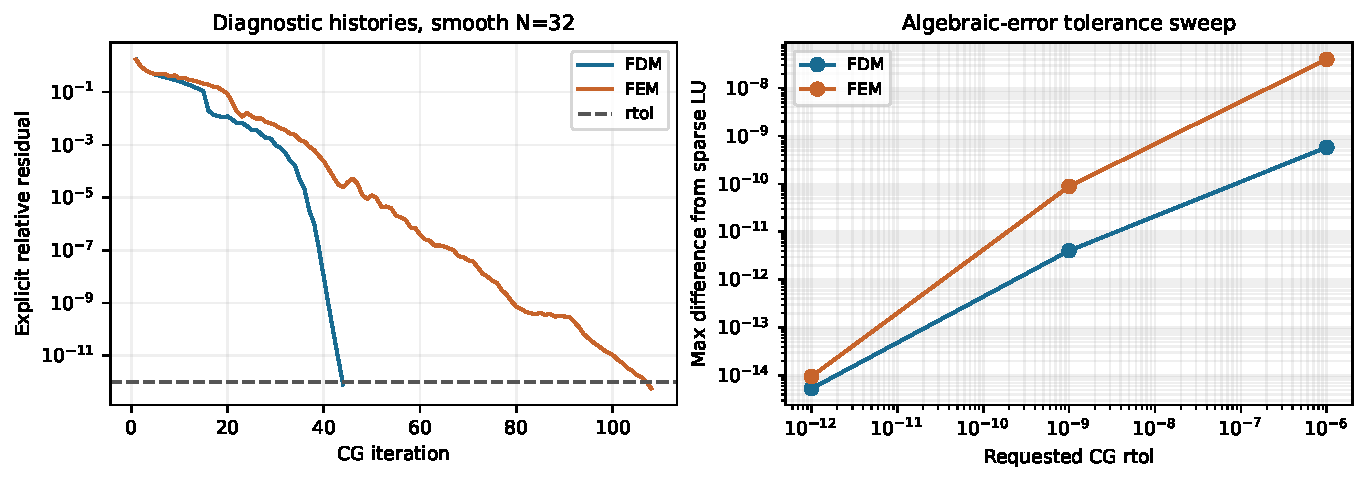
\includegraphics[width=0.95\linewidth]{figures/fig06_solver_validation.pdf}
\caption{Explicit residual histories and solution agreement with the direct reference. History collection performs additional matrix-vector products and is excluded from the main timing comparison.}
\end{figure}

\begin{table}[H]\centering\small
\begin{tabular}{llrrrrr}
\toprule
Method & $N$ & DOF & $E_{2,h}$ & $E_\infty$ & $p_{2,h}$ & CG its.\\
\midrule
FDM & 16 & 225 & 1.598e-03 & 3.205e-03 & --- & 19\\
FDM & 32 & 961 & 3.988e-04 & 8.009e-04 & 2.00 & 44\\
FDM & 64 & 3969 & 9.966e-05 & 2.003e-04 & 2.00 & 94\\
FDM & 128 & 16129 & 2.491e-05 & 5.007e-05 & 2.00 & 192\\
FEM & 16 & 225 & 1.614e-03 & 3.214e-03 & --- & 53\\
FEM & 32 & 961 & 4.042e-04 & 8.079e-04 & 2.00 & 108\\
FEM & 64 & 3969 & 1.011e-04 & 2.021e-04 & 2.00 & 225\\
FEM & 128 & 16129 & 2.527e-05 & 5.053e-05 & 2.00 & 443\\
\bottomrule
\end{tabular}

\caption{Computed four-mesh validation for both implementations. $p_{2,h}$ is the successive-grid rate in the nodal area-weighted norm. The CSV also contains continuous reconstructed errors, maximum-norm rates and residuals.}
\label{tab:alg_smooth}
\end{table}

\begin{figure}[H]\centering
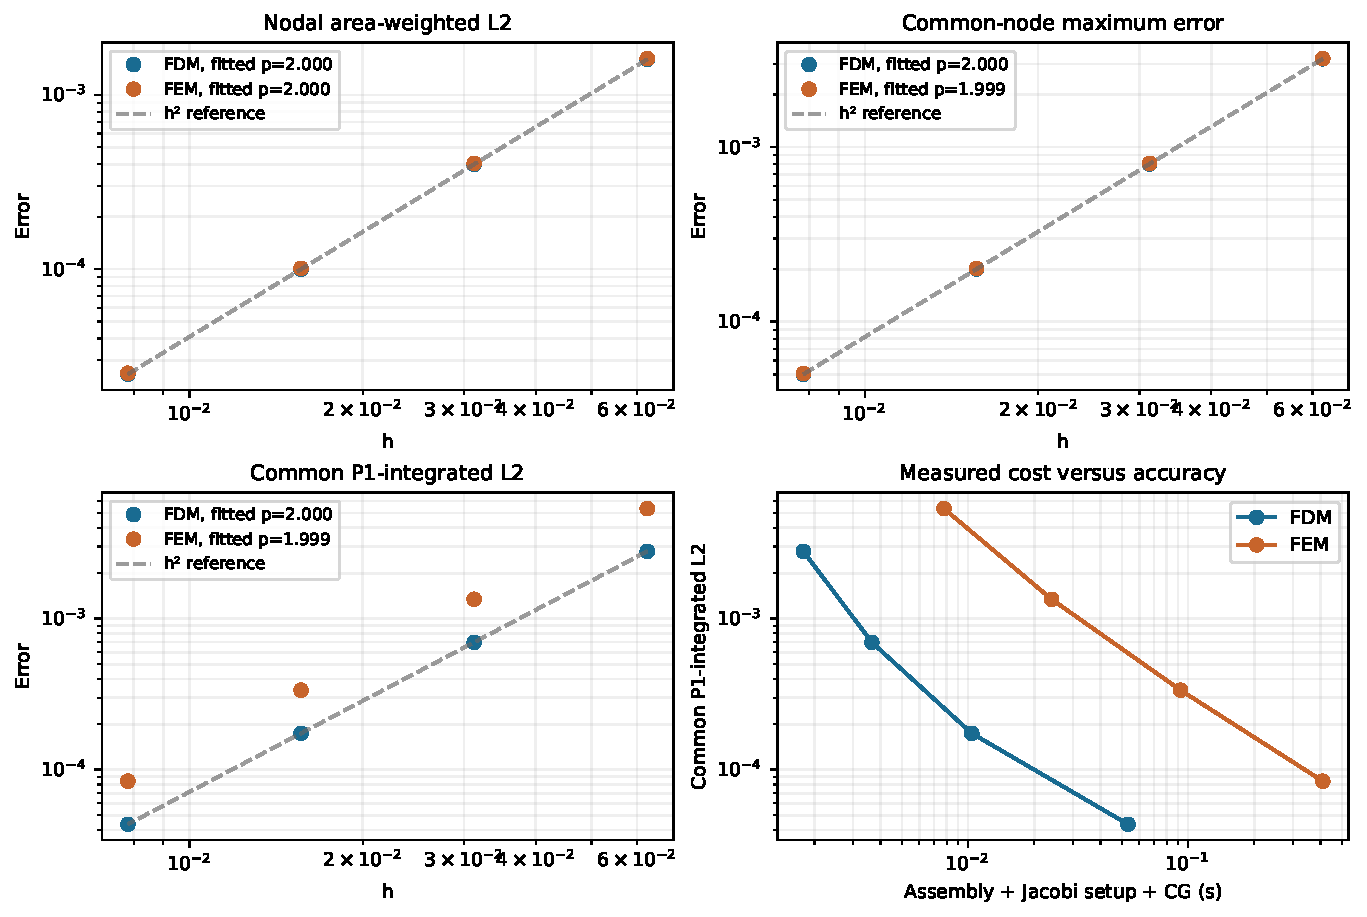
\includegraphics[width=0.91\linewidth]{figures/fig03_accuracy_cost.pdf}
\caption{Refinement checks in two nodal norms and a common integrated norm, with the measured assembly-and-CG cost. Fitted orders use the finest three meshes; the dashed lines show the theoretical quadratic slope. Timings are local CPU measurements.}
\end{figure}

\begin{table}[H]\centering\small
\begin{tabular}{lrrrrr}
\toprule
Method & $N$ & nnz & Assembly (s) & CG (s) & LU (s)\\
\midrule
FDM & 64 & 19593 & 2.302e-03 & 7.916e-03 & 1.878e-02\\
FDM & 128 & 80137 & 8.426e-03 & 4.431e-02 & 9.600e-02\\
FEM & 64 & 19593 & 7.319e-02 & 1.904e-02 & 1.970e-02\\
FEM & 128 & 80137 & 3.072e-01 & 1.017e-01 & 9.136e-02\\
\bottomrule
\end{tabular}

\caption{Median stage costs from three repetitions. CG excludes Jacobi setup in this table; LU includes factorisation and one triangular solve. The cost--accuracy plot additionally includes assembly and Jacobi setup.}
\end{table}

\subsection{Interface diagnostics and coefficient contrast}
All fluxes use the common $+x$ normal and the physical sign $q_x=-a\partial_xu$. For FDM the code forms the shared edge fluxes directly from the face arrays. Their discrete divergence checks the assembled local balance. The interface flux error is measured against $q_*=-2c/(1+c)$. To quantify a two-sided flux difference, the code also evaluates the nearest pure-material edge on each side and reports the maximum difference at common $y$ values. These two edges are a distance $h$ apart from the interface. This reconstruction is exact for the piecewise-linear benchmark, and its location is explicit in the implementation.

The arithmetic scheme retains shared-face conservation. Its inaccurate interface resistance can alter the numerical solution and physical flux. The plots and data report the actual errors. The magnitude of a reconstructed jump depends on the reconstruction and boundary data. The raw FEM traces are evaluated on the two triangles adjacent to each aligned interface segment, sorted by segment midpoint.

In this experiment the arithmetic scheme also gives a very small two-sided reconstructed jump, while its shared interface flux has a substantial error against the exact flux (Table~\ref{tab:alg_interface}). Checking the jump alone would therefore miss the interface resistance defect. Harmonic nodal exactness refers to nodal values; plain P1 interpolation across an unresolved interface introduces an additional interpolation error in a continuous norm.

\begin{table}[H]\centering\small
\begin{tabular}{llrrrr}
\toprule
Method & Face rule & $N$ & $E_\infty$ & $E_q$ & $J_q$\\
\midrule
FDM & arithmetic & 63 & 9.600e-03 & 6.619e-01 & 3.846e-13\\
FDM & harmonic & 63 & 7.327e-15 & 1.081e-13 & 6.015e-13\\
FEM & element integral & 64 & 3.308e-14 & 5.167e-13 & 4.619e-13\\
\bottomrule
\end{tabular}

\caption{Layered diagnostics at neighbouring mesh sizes, $c=10$. $E_q$ is the maximum interface flux error; $J_q$ is the explicitly defined two-sided flux difference. Mesh parity follows each method's interface treatment.}
\label{tab:alg_interface}
\end{table}

\begin{figure}[H]\centering
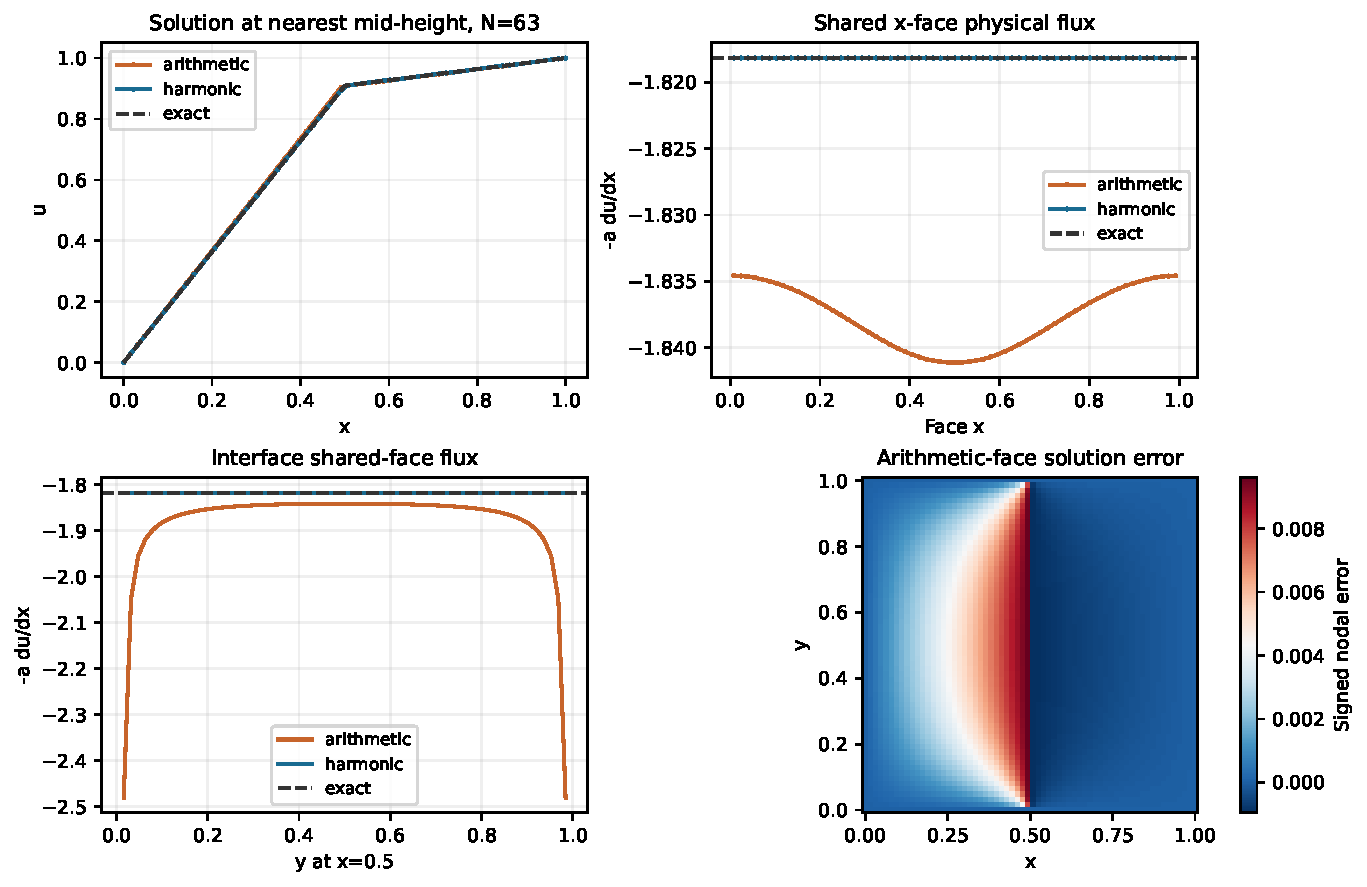
\includegraphics[width=0.90\linewidth]{figures/fig04_interface.pdf}
\caption{Computed layered FDM fields at $N=63$. The lower-left panel displays the shared interface flux along $y$, with prescribed top and bottom boundary edges excluded. The error map shows how an interface conductance defect affects the two-dimensional solution.}
\end{figure}

For conditioning, the harmonic FDM matrix is tested at $N=15,31,63$ and $c=1,10,100$. The smallest eigenvalue is estimated using shift-invert Lanczos with shift zero; the largest uses the largest-algebraic option. The reported estimate is $\widehat\kappa_2=\widehat\lambda_{\max}/\widehat\lambda_{\min}$. Explicit eigenpair residuals accompany each estimate. CG iteration counts are recorded with and without Jacobi at comparable explicit relative residuals. These data concern the unscaled Dirichlet-eliminated FDM matrix. The analytical contrast-dependent bound remains an upper bound; the experiments measure the behaviour for this coefficient geometry.

\begin{figure}[H]\centering
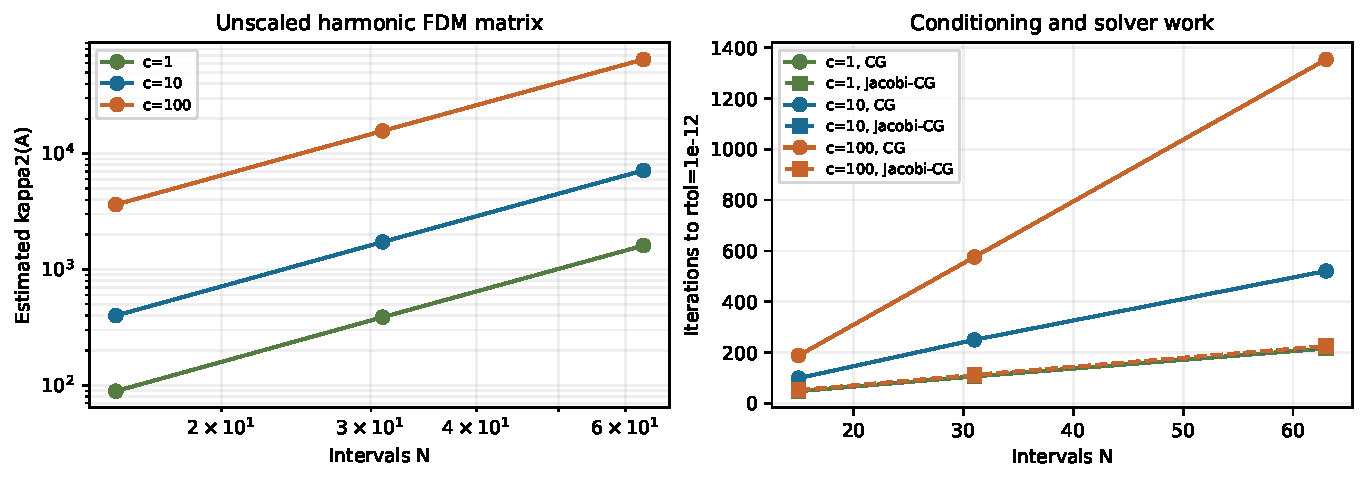
\includegraphics[width=0.95\linewidth]{figures/fig05_conditioning.pdf}
\caption{Estimated conditioning and actual CG work under mesh refinement and coefficient contrast. Jacobi changes the iterative system, while the left panel always refers to the original matrix.}
\end{figure}

\subsection{Reproduction and integration}
\texttt{python -B run\_all.py} reruns the checks, numerical experiments, tables and six figures from the configuration file. The implementation uses double precision. The supplied PDF is a standalone reading version; \texttt{algorithm\_section.tex} can be included as Section~3 after the supplied Method section. The folder contains the numerical source, tests, raw CSV tables, representative field arrays, figures in PDF/PNG, and software provenance. The existing interface-PINN experiment is available as a separate advanced supplement, with its own training outputs and architecture limitations.

\bibliographystyle{plain}
\bibliography{refs}
\end{document}
